%Imports and headers
\documentclass[a4paper]{article}  %Or use titlepage

%% Language and font encodings
\usepackage[english]{babel}
\usepackage[utf8]{inputenc}
\usepackage[T1]{fontenc}
\usepackage{float} %makes you be able to use H option, places fig there and only there. VERY useful

%% Sets page size and margins
\usepackage[a4paper,top=3cm,bottom=2cm,left=3cm,right=3cm,marginparwidth=1.75cm]{geometry}

%% Useful packages
\usepackage{amsmath}
\usepackage{graphicx}
\usepackage[colorinlistoftodos]{todonotes}
\usepackage[colorlinks=true, allcolors=blue]{hyperref}

%% Extra packages for color and stuff
\usepackage{geometry}
\usepackage{xcolor}
\usepackage{amsmath}
\usepackage[some]{background}

%% Header, foot and page number in bottom right corner
\usepackage{fancyhdr}
\usepackage{lipsum}

% For gantt chart
\usepackage{pgfgantt}

%% For long comments
\usepackage{comment}

% Turn on the style
\pagestyle{fancy}
% Clear the header and footer
\fancyhead{}
\fancyfoot{}

% The file containing our references, in BibTeX format
\usepackage{csquotes} % Recommended by biblatex
\usepackage[style=numeric,sorting=none,backend=biber]{biblatex}
\addbibresource{references.bib}

%%%%% Title page
\begin{document}
\thispagestyle{empty}
\begin{titlepage}
\title{\vspace{60mm} \bf
        Project plan BB200X\\
        \large Containerization of microbial \\
        protoeomics data processing pipelines
}  %Fix to center title vertically
\author{Timothy Bergström}
\maketitle
\thispagestyle{fancy}  %Page number for title (\maketitle clears foot and head, so it needs to be after it)
\vspace*{\fill}
\centering{tib@kth.se \\ 950502-1312 \\ KTH: Royal institute of technology}
\end{titlepage}

\newpage

%%%%% Table of contents
\thispagestyle{empty}
\tableofcontents
\newpage

%%%%% Chapters
% set footer
% Set the right side of the footer to be the page number
\fancyfoot[R]{\thepage}  % Page number
\fancyfoot[L]{\date{\today}}  % date on footer
\fancyhead[C]{BB200X - Project plan}  % Text on head
\setcounter{page}{1}

% document
\section{Introduction}

Mass spectrometry (MS)-based Proteomics is currently the most comprehensive technique to analyze protein content in biological samples. Modern MS generate vast amounts of data and the analysis of such data is generally considered as a bottleneck, both due to the volume of data but also as the methods for processing the data are complex and need manual intervention. As it is hard to recreate the exact software environment used during processing, the majority of all results produced with mass spectrometers cannot be accurately reproduced outside of the lab where it was initially generated.

Containerization and workflow management is a way to remedy the situation. Containerization is a technique to install software, not into a particular computer, but into a virtual container environment, in a so-called image. The image can be distributed to several separate computers, yet guaranteed to execute in the exact same way regardless of the operating system. There are several such containerization techniques available. Here, we will focus on one named Singularity, as it is the preferred solution of most HPC clusters, such as UPPMAX.

The second concept, workflow management, deals with how different pieces of dependent software can be consequently executed in a particular environment. Again, there are several workflow managers available, but we will focus on one named NextFlow as it currently is a preferred solution for sequencing data at SciLifeLab.

The aim of the project is to utilize containerization to embed a software named \textit{Quandenser}, a newly created software made in SciLifeLab by Lukas Käll and Matthew The, which condenses quantification data from label-free MS experiments \cite{quandenser}. In unison with several other software embedded in the container, a workflow is to be created based on Nextflow with the aim to analyze MS generated data to protein quantification results.

%\newpage
\section{Objectives}

The main objectives for the project are as follows:
\begin{enumerate}
\item Develop a Singularity container for the software \textit{Quandenser}, which processes label-free MS data for protein quantification \cite{quandenser}.
\item A NextFlow pipeline, which will integrate the singularity container produced in the previous step.
\item Apply the data for two different microbial datasets generated in Paul Hudson’s lab using tandem-MS, one of which was created by growing cyanobacteria under different conditions \cite{michael}. The microbial data sets were generated by analyzing the proteome of two different lithotrophic bacteria.
\end{enumerate}

%\newpage
\section{Work Breakdown Structure}

A Work Breakdown Structure is a method to visualize the workflow of the project. In the figure below, a full breakdown of the project is shown.

\begin{figure}[H]
    \centering
    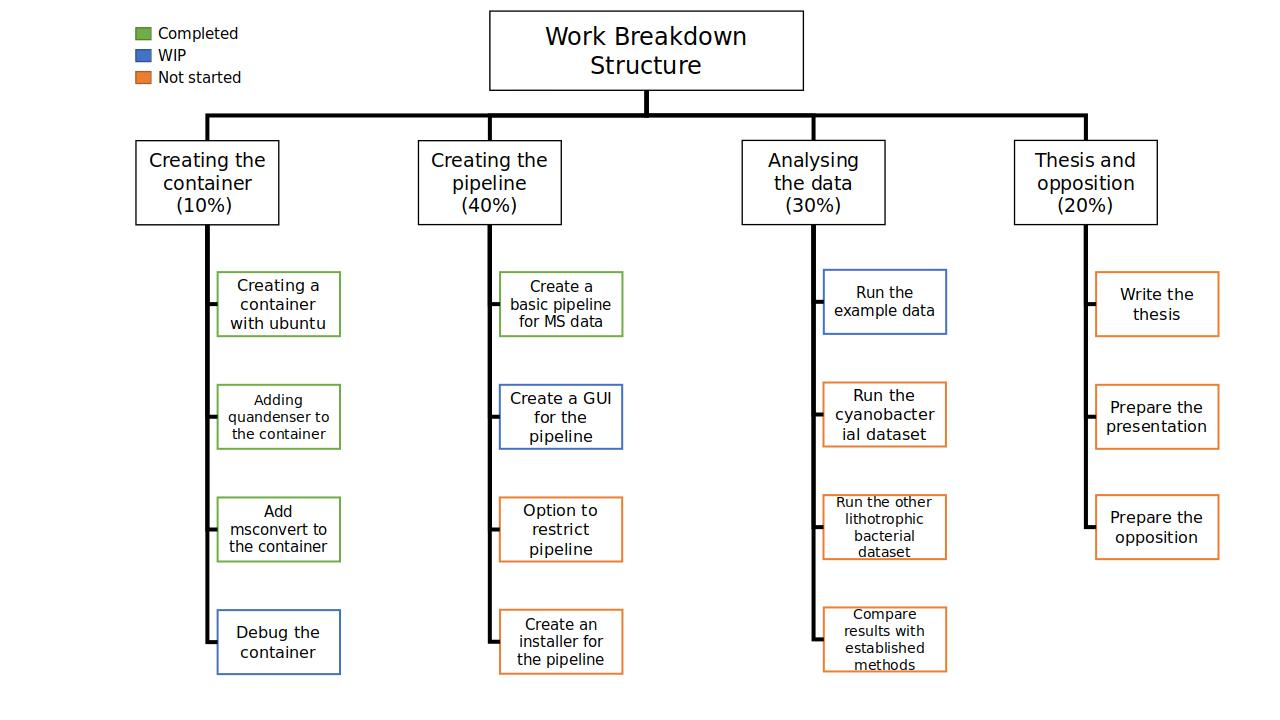
\includegraphics[width=\textwidth,height=\textheight,keepaspectratio]{Pictures/wbs.jpg}
    \caption{Work Breakdown Structure of the project. The percentages are the allocated time for each part of the project. The colors indicate which parts have been completed, are currently worked on or have not been started yet}
\end{figure}

%\newpage
\section{Milestones}

The milestones are ordered in the same order which they are expected to be completed.

\begin{enumerate}
\item Create a container, which can run Quandenser (FINISHED)
\item Create a basic pipeline with nextflow, integrating the container (FINISHED)
\item Run an example data set on the pipeline (FINISHED)
\item Finish a basic UI for the pipeline, to speed up the process when running the pipeline (FINISHED)
\item Make an installer for the pipeline, which automatically installs the dependencies for running the pipeline (FINISHED)
\item Integrate a "restricted" pipeline, so the user can choose where to begin and stop (FINISHED)
\item Run the cyanobacterial data set on the pipeline (FINISHED)
\item Run the other bacterial data set on the pipeline
\item Create visual comparisons between the pipeline and protein quantification with established methods
\item Finished the thesis
\item Opposition report finished
\item Final presentation
\end{enumerate}

%\newpage
\section{Timeplan}

A gantt chart is shown in the figure below, explaining the time plan of the project.

\definecolor{barblue}{RGB}{153,204,254}
\definecolor{groupblue}{RGB}{51,102,254}
\definecolor{linkred}{RGB}{165,0,33}
\renewcommand\sfdefault{phv}
\renewcommand\mddefault{mc}
\renewcommand\bfdefault{bc}
\setganttlinklabel{s-s}{START-TO-START}
\setganttlinklabel{f-s}{FINISH-TO-START}
\setganttlinklabel{f-f}{FINISH-TO-FINISH}
\sffamily
\makebox[\textwidth]{
\begin{ganttchart}[
    canvas/.append style={fill=none, draw=black!5, line width=.75pt},
    hgrid style/.style={draw=black!5, line width=.75pt},
    vgrid={*1{draw=black!5, line width=.75pt}},
    today=2,
    today rule/.style={
      draw=black!64,
      dash pattern=on 3.5pt off 4.5pt,
      line width=1.5pt
    },
    today label font=\small\bfseries,
    title/.style={draw=none, fill=none},
    title label font=\bfseries\footnotesize,
    title label node/.append style={below=7pt},
    include title in canvas=false,
    bar label font=\mdseries\small\color{black!70},
    bar label node/.append style={left=2cm},
    bar/.append style={draw=none, fill=black!63},
    bar incomplete/.append style={fill=barblue},
    bar progress label font=\mdseries\footnotesize\color{black!70},
    group incomplete/.append style={fill=groupblue},
    group left shift=0,
    group right shift=0,
    group height=.5,
    group peaks tip position=0,
    group label node/.append style={left=.6cm},
    group progress label font=\bfseries\small,
    link/.style={-latex, line width=1.5pt, linkred},
    link label font=\scriptsize\bfseries,
    link label node/.append style={below left=-2pt and 0pt}
  ]{1}{20}
  \gantttitle[title label node/.append style={below left=7pt and -3pt}]{WEEKS:\quad1}{1}
  \gantttitlelist{2,...,20}{1} \\
  \ganttgroup[progress=75]{Creating the container}{1}{10} \\
  \ganttbar[progress=100, name=WBS1A]{\textbf{Creating a container with ubuntu}}{1}{1} \\
  \ganttbar[progress=100,name=WBS1B]{\textbf{Add quandenser to the container}}{2}{3} \\
  \ganttbar[progress=100,name=WBS1C]{\textbf{Add msconvert to the container}}{2}{3} \\
  \ganttbar[progress=30,name=WBS1D]{\textbf{Debug the container}}{3}{7} \\[grid]
  \ganttlink[link type=f-s]{WBS1A}{WBS1B}
  \ganttgroup[progress=25]{Creating the pipeline}{1}{10} \\
  \ganttbar[progress=100, name=WBS2A]{\textbf{Create a basic pipeline for MS data}}{1}{3} \\
  \ganttbar[progress=10, name=WBS2B]{\textbf{Create a GUI for the pipeline}}{3}{6} \\
  \ganttbar[progress=0, name=WBS2C]{\textbf{Options to restrict pipeline}}{7}{9} \\
  \ganttbar[progress=0, name=WBS2D]{\textbf{Create an installer for the pipeline}}{9}{10} \\[grid]
  \ganttlink[link type=f-f]{WBS2B}{WBS2D}
  \ganttgroup[progress=5]{Analysing the data}{10}{20} \\
  \ganttbar[progress=10, name=WBS3A]{\textbf{Run the example data}}{11}{11} \\
  \ganttbar[progress=0, name=WBS3B]{\textbf{Run the cyanobacterial data set}}{12}{17} \\
  \ganttbar[progress=0, name=WBS3C]{\textbf{Run the other lithotrophic bacterial data set}}{12}{17} \\
  \ganttbar[progress=0, name=WBS3D]{\textbf{Compare results with established methods}}{13}{17} \\[grid]
  \ganttlink[link type=f-f]{WBS3B}{WBS3D}
  \ganttgroup[progress=0]{Thesis and opposition}{11}{20} \\
  \ganttbar[progress=0, name=WBS4A]{\textbf{Write the thesis}}{10}{19} \\
  \ganttbar[progress=0, name=WBS4B]{\textbf{Write opposition}}{19}{19} \\
  \ganttbar[progress=0, name=WBS4C]{\textbf{Prepare presentation}}{15}{20} \\
  \ganttlink[link type=s-f]{WBS4A}{WBS4C}
\end{ganttchart}
}

%\newpage
\section{MoSCoW}

The MoSCoW method is a way to structure and prioritize tasks in a project. MoSCow is an acronym for "Must, Should, Could and Won't. In this case, Must is what must be fulfilled for the project to be completed. Should is what should to be fulfilled to improve the quality of the project. Could is extra features or analyses that could be done. Won't is anything that won't be performed in the project\\

{\Large MUST}
\begin{itemize}
  \item Create a functional container for the project
  \item Create a pipeline for the container
\end{itemize}

{\Large SHOULD}
\begin{itemize}
  \item Design and create a GUI (graphical user interface) for the pipeline, for easy usage
  \item Analyze the microbial data sets with the pipeline
\end{itemize}

{\Large COULD}
\begin{itemize}
  \item Also create a CLI (command line interface) for the pipeline, to work without visual
  \item Run the pipeline on other data sets than the microbial data (ex a human proteome)
\end{itemize}

{\Large WON'T}
\begin{itemize}
  \item Try other established method
  \item Create my own label-free software
\end{itemize}

%\newpage
\section{Business case}

\subsection{Scientific aspects}

Improved tools for scientific research are constantly needed in the academic world.

\subsection{Societal aspects}



\subsection{Financial aspects}

The project is built from open-source programs, which will make it difficult to make the project \textit{commercially} viable. However, the main targets would be researchers in the academic world,dependency is under Apache License Version 2.0, which states that you are allowed to use the software for commercial purposes,

%\newpage
\section{Stakeholder analysis}

A stakeholder analysis is a way to visualize which people will benefit from the project and their interests in the completion of the project.

\newcommand{\textone}{Lukas Käll is the supervisor of the project. His interest in the project is the highest, due to him being the creator of the program "Quandenser" alongside Matthew The. Creating an easy to use pipeline will make more researcher willing to switch over from their old tools to the new one which he has created}
\newcommand{\texttwo}{Peter Savolainen is the examiner of the project. His interest is to oversee the project as a whole to ensure that the project is finished in time}
\newcommand{\textthree}{Michael Jahn holds the data for the microbial data sets. His interests are that improved tools for analysis might yield more accurate results, thus making his research more precise}
\newcommand{\textfour}{ScilifeLaboratory is where the project is taking place. Researchers in SciLife might have some use for the end product of the project}
\newcommand{\textfive}{KTH is the main institution, which is interested in giving students their degree when they are finished}
\newcommand{\textsix}{A small area of science would benefit from the project, if I manage to create an easy to use pipeline which show superior performance for label-free quantification. Thus, their research could be improved by more accurate quantification tools}
\newcommand{\textseven}{Socieity does not have a large influence on the project, but improvements from the research with the pipeline might have a positive impact in the long run.}

\begin{table}[H]
\large
\resizebox{\textwidth}{!}{
\begin{tabular}{|p{4cm}|p{9cm}|}
\hline
Primary stakeholder & Description\\ \hline
Lukas Käll & \textone \\
Peter Savolainen & \texttwo \\
Michael Jahn & \textthree \\
ScilifeLaboratory & \textfour \\
KTH & \textfive \\
 & \\
 & \\ \hline
Secondary stakeholder & Description \\ \hline
Researchers & \textsix \\
Society & \textseven \\ \hline
\end{tabular}}
\caption{Stakeholder analysis}
\end{table}

%\newpage
\section{Risk assessment}

There are some risks which might prevent the project from completing. In the table below, some of the risks are assessed on the likelihood that it happens, the impact of the risk and how to prevent the risk from happening or how to lowere the impact.

\begin{table}[H]
\large
\resizebox{\textwidth}{!}{
\begin{tabular}{|p{3cm}|p{1.8cm}||p{1.3cm}||p{7cm}|}
\hline
Risk & Likelihood & Impact & Prevention\\ \hline
Work computer breaking down & Low & High & Store the project on github and the main files on an external hard-drive \\
Incompatible data from microbial set & Medium & Medium & The underlying software should be able to handle most of the data and if not, integrate the packaged conversion program to fix the data. \\
Unfixable errors in the underlying programs & High & Medium & Find a workaround for the program and if possible, use another program instead \\
Sickness & High & Low & Most of the work is on github and I can run the analyses on a data cluster, so I can easily work from home if I get sick. \\
\hline
\end{tabular}}
\caption{Risk assessment}
\end{table}

%\newpage
\section{SWOT}

The main strengths of the project are:\\
The supervisor has a lot of knowledge about the software used, since he wrote "Quandenser", which is the cornerstone of the pipeline. The working environment is also very good in Scilife, making the work efficient. I also have access to a good computer, which can handle the computationally demanding processing of the data.

The weaknesses are that I have a limited knowledge about the program used, which will require more practice and learning. Every program I use is also completely new, meaning that I have to learn everything from scratch.

The opportunities are plenty. I will learn a lot during my time on the project and my ability to implement and create tools will also improve during the time at Scilife.

The threats are few, but can have a large impact on the project. The data sets are large and might require too much time to process on the data clusters, thus I run the risk of running out of calculation time. Some programs I use are built on old frameworks, which have long been deprecated, meaning some issues might be unfixable and I might need to take another approach.

\begin{figure}[H]
    \centering
    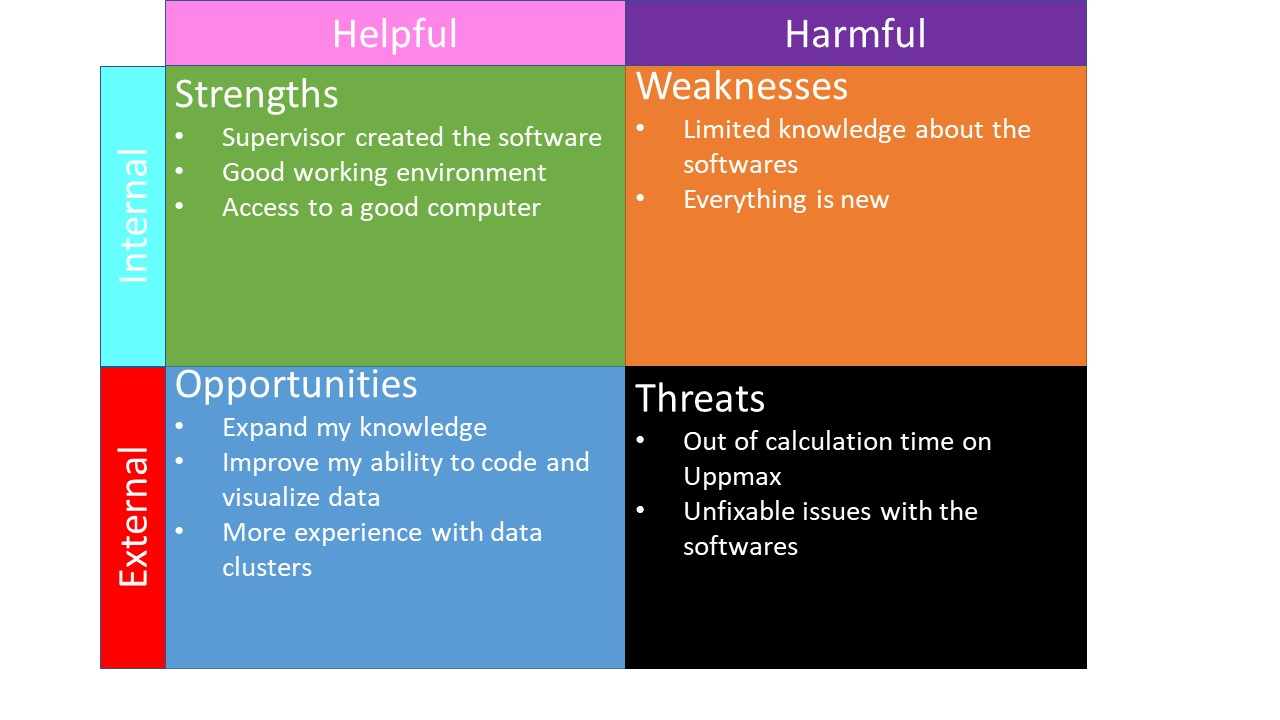
\includegraphics[width=\textwidth,height=\textheight,keepaspectratio]{Pictures/SWOT.jpg}
    \caption{SWOT analysis}
\end{figure}

\newpage
\printbibliography


\end{document}
